\documentclass[hyperref]{ctexart}
\usepackage[top=1.5cm,left=1.5cm,right=1.5cm,bottom=1.5cm]{geometry}
\usepackage[utf8]{inputenc}
\usepackage{graphicx}
\usepackage{xcolor}
\usepackage{fontawesome}
\usepackage{tikz}
\usepackage{mathptmx}
\pagestyle{empty}
\setlength{\parindent}{0pt} 

%定义
\newcommand{\information}[2]{
{\zihao{5}  \color{orange}  #1}\hspace{0.2em} #2 \hspace{0.5em}
}
%定义
\newcommand{\partskip}{\bigskip\bigskip}
%定义
\newcommand{\wenxiannumber}[1]{
\makebox[0pt][l]{{\color{orange}\faCircle} }\hspace{0.17em}\textcolor{white}{\textbf{#1}}\hspace{0.1em}
}

%声明
\pgfdeclarehorizontalshading{myshadingA}{0.15cm} {color(0cm)=(orange); color(17cm)=(white)}
\begin{document}

%%%%%%%%%%%%%%%%%%%%%%%%%%%%%%%%%%header%%%%%%%%%%%%%%%%%%%%%%%%%%%%%%%%%%%
\begin{minipage}[b][3cm][t]{0.7\linewidth}
{\zihao{-0} \heiti 甘云汉 }\\[0.7em]
\information{\faEnvelope}{hank.gan@foxmail.com}\\
%\information{\faTwitter}{@example}%
\information{\faMapMarker}{湖北省武汉市洪山区}\\
\information{\faGlobe}{\url{https:www.amghank.cn}}\\
\information{ \faPhone}{18871007081} \\
\end{minipage}
\hfill
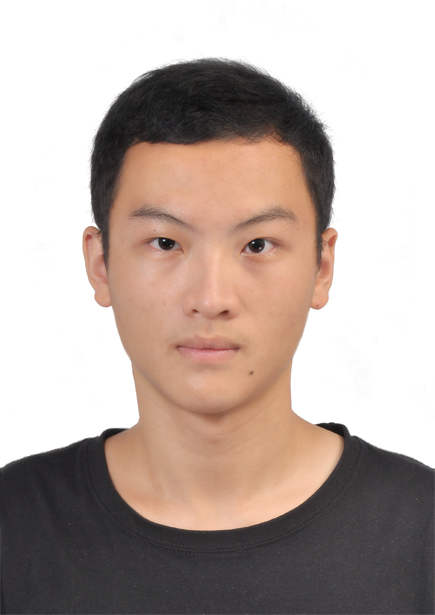
\includegraphics[height=3cm]{证件照.jpg}

%%%%%%%%%%%%%%%%%%%%%%%%%%%%%%%%%%body%%%%%%%%%%%%%%%%%%%%%%%%%%%%%%%%%%%
%%%%%%%%%%%%%%%%%%%%%%%%%%%%%%%%%%教育背景%%%%%%%%%%%%%%%%%%%%%%%%%%%%%%%%%%%
\partskip

{\zihao{2} \heiti 教育背景 }

\pgfuseshading{myshadingA} 

\smallskip
{ \color{orange}\faHeartbeat} \quad \textbf{武汉理工大学} \quad{电子科学与技术} \quad{GPA:3.603/5} \quad{CET-6}
\quad 综合排名:8/118
\hfill  \makebox[3cm][l]{2018 年至今}

\quad \quad 主攻方向:{\kaishu 嵌入式应用、Cortex-M系列内核、FPGA逻辑设计、SOC架构}

\quad \quad 期望研究方向:{\kaishu 数字IC/SOC设计、可重构计算、处理器架构、并行加速}

%%%%%%%%%%%%%%%%%%%%%%%%%%%%%%%%%%科研项目%%%%%%%%%%%%%%%%%%%%%%%%%%%%%%%%%%%
\partskip

{\zihao{2} \heiti 科研项目 }

\pgfuseshading{myshadingA} 

\smallskip
{ \color{orange}\faHeartbeat}\quad 电推平底船的气泡减阻自动控制系统
\hfill  \makebox[3cm][l]{$2020$年}

\quad \quad {\kaishu 利用训练好的 BP 神经网络自动调整船舶微气泡减阻所需的气泡量,实现嵌入式自动控制}

\smallskip
{ \color{orange}\faHeartbeat}\quad 非接触式口罩识别及温度监测系统
\hfill  \makebox[3cm][l]{$2020$年}

\quad \quad {\kaishu 利用高云 FPGA 作为逻辑控制器进行红外测温,同时利用 K210 进行人脸识别和口罩检测}

\smallskip
{ \color{orange}\faHeartbeat}\quad 基于 Cortex-m3 内核的语音识别声源定位加速器
\hfill  \makebox[3cm][l]{$2021$年}

\quad \quad {\kaishu 2021 第五届集成电路创新设计大赛 ARM 杯项目,自制算法 IP}
%%%%%%%%%%%%%%%%%%%%%%%%%%%%%%%%%%获奖&荣誉%%%%%%%%%%%%%%%%%%%%%%%%%%%%%%%%%%%
\partskip

{\zihao{2} \heiti 荣誉证书 }

\pgfuseshading{myshadingA} 

\smallskip
{ \color{orange}\faHeartbeat}\quad “赛迪环保杯”第十三届节能减排大赛全国二等奖 \hfill \makebox[3cm][l]{$2019-2020$年}

\smallskip
{ \color{orange}\faHeartbeat}\quad “Ti 杯”电子设计大赛湖北省一等奖 \hfill \makebox[3cm][l]{$2020$年 }

\smallskip
{ \color{orange}\faHeartbeat}\quad  第四届全国大学生 FPGA 创新设计大赛二等奖 \hfill \makebox[3cm][l]{$2020$年}

\smallskip
{ \color{orange}\faHeartbeat}\quad  武汉理工大学校二等奖学金 \hfill \makebox[3cm][l]{$2020$年}

\smallskip
{ \color{orange}\faHeartbeat}\quad  “挑战杯·中国银行”大学生课外学术科技作品竞赛湖北省特等奖 \hfill \makebox[3cm][l]{$2021$年}

\smallskip
{ \color{orange}\faHeartbeat}\quad  全国大学生集成电路创新设计大赛ARM杯  全国一等奖第一名(ARM企业杯) \hfill \makebox[3cm][l]{$2021$年}

%%%%%%%%%%%%%%%%%%%%%%%%%%%%%%%%%%技能%%%%%%%%%%%%%%%%%%%%%%%%%%%%%%%%%%%
\partskip

{\zihao{2} \heiti 专业技能 }

\pgfuseshading{myshadingA}

\smallskip
{ \color{orange}\faHeartbeat}\quad 软件:
\fcolorbox{gray!40}{white}{C} \hspace{0.3em}
\fcolorbox{gray!40}{white}{tcl} \hspace{0.3em}
\fcolorbox{gray!40}{white}{Python} \hspace{0.3em}

\smallskip
{ \color{orange}\faHeartbeat}\quad 硬件:
\fcolorbox{gray!40}{white}{Verilog HDL} \hspace{0.3em}
\fcolorbox{gray!40}{white}{STM32/Cortex-M3} \hspace{0.3em}
\fcolorbox{gray!40}{white}{FPGA/ZYNQ} \hspace{0.3em}
\hspace{0.3em} 

\smallskip
{ \color{orange}\faHeartbeat}\quad 语言能力:英语有良好的读写能力、通过CET-4和CET-6.


\end{document}





